\documentclass[dvipdfmx]{jarticle}
\pagestyle{empty}
\usepackage{tikz}
\usetikzlibrary{shapes,calc}
\begin{document}
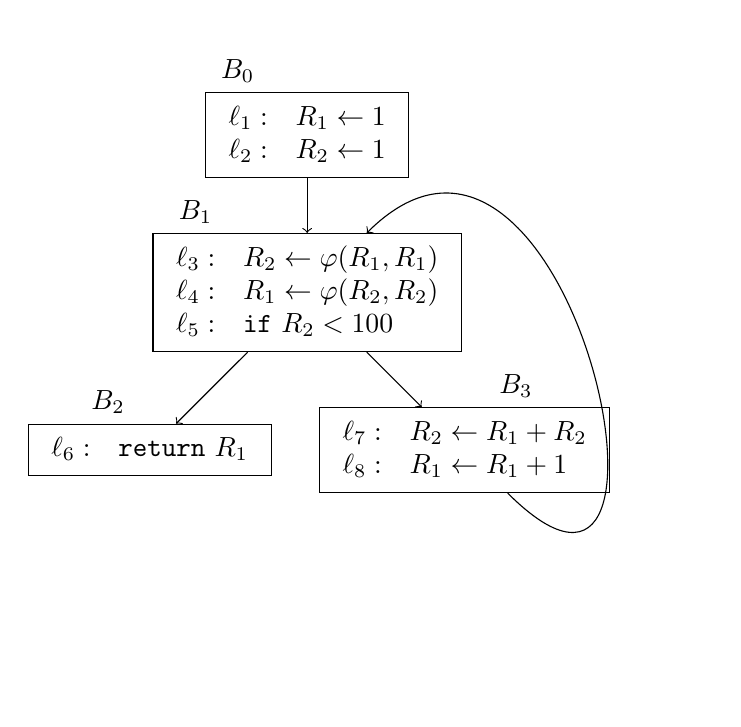
\begin{tikzpicture}
\node[draw,label={135:{$B_0$}}] (N1) at (0,0) {$\begin{array}{ll}
    \ell_1: & R_1\leftarrow 1\\
    \ell_2: & R_2\leftarrow 1\end{array}$};
\node[draw,label={145:{$B_1$}}] (N2) at (0,-2) {$\begin{array}{ll}
    \ell_3: & R_2\leftarrow\varphi(R_1,R_1)\\
    \ell_4: & R_1\leftarrow\varphi(R_2,R_2)\\
    \ell_5: & \texttt{if}\ R_2<100
\end{array}$};
\node[draw,label={120:{$B_2$}}] (N3) at (-2,-4) {$\begin{array}{ll}
    \ell_6: & \texttt{return}\ R_1
\end{array}$};
\node[draw,label={60:{$B_3$}}] (N4) at (2,-4) {$\begin{array}{ll}
    \ell_7: & R_2\leftarrow R_1+R_2\\
    \ell_8: & R_1\leftarrow R_1+1
\end{array}$};
\path[->] (N1) edge (N2) (N2) edge (N3) (N2) edge (N4);
\path[->] (N4) edge [out=315,in=45,looseness=2.5] (N2);
\end{tikzpicture}
\end{document}